%% ============================================================================
%%  A Self-Improving Cyber-Physical Data Engine for Annotation-Free
%%  Sponsor-Logo Analytics in Sports Broadcasts
%%
%%  Target venue : IEEE International Conference on Cyberworlds (CW)
%%  Format       : IEEEtran conference, 2-column.  Compile on Overleaf or:
%%                   latexmk -pdf main.tex
%%
%%  NOTE ON NUMBERS:  All quantitative results are marked \TODOnum{...} and are
%%  PLACEHOLDERS to be replaced with measured values.  Do NOT submit as-is.
%% ============================================================================
\documentclass[conference]{IEEEtran}
\IEEEoverridecommandlockouts

\usepackage{cite}
\usepackage{amsmath,amssymb,amsfonts}
\usepackage{graphicx}
\usepackage{booktabs}
\usepackage{xcolor}
\usepackage{url}
\usepackage[colorlinks=true,allcolors=blue]{hyperref}
\usepackage{tikz}
\usepackage{pgfplots}
\pgfplotsset{compat=1.18}
\usetikzlibrary{positioning,arrows.meta,shapes.geometric,fit,backgrounds,calc}

% --- placeholder helper: makes unfilled numbers visually obvious -------------
\newcommand{\TODOnum}[1]{{\color{red}\textbf{#1}}}

% --- shared tikz styles ------------------------------------------------------
\tikzset{
  blk/.style   ={rectangle, rounded corners=2pt, draw=black!70, thick,
                 fill=blue!6, align=center, inner sep=4pt, font=\scriptsize,
                 minimum height=8mm, text width=22mm},
  data/.style  ={rectangle, draw=black!55, fill=gray!8, align=center,
                 inner sep=3pt, font=\scriptsize\itshape, text width=20mm},
  teach/.style ={blk, fill=orange!12},
  stud/.style  ={blk, fill=green!12},
  arr/.style   ={-{Stealth[length=2mm]}, thick, draw=black!65},
}

\begin{document}

\title{A Self-Improving Cyber-Physical Data Engine for\\
Annotation-Free Sponsor-Logo Analytics in Sports Broadcasts}

\author{\IEEEauthorblockN{First Author\IEEEauthorrefmark{1},
Second Author\IEEEauthorrefmark{1}, Third Author\IEEEauthorrefmark{2}}
\IEEEauthorblockA{\IEEEauthorrefmark{1}Affiliation One,
\IEEEauthorrefmark{2}Affiliation Two\\
\texttt{\{author1,author2\}@inst.edu}}}

\maketitle

% ============================================================================
\begin{abstract}
Sponsor-logo analytics in sports broadcasts traditionally requires annotating
thousands of frames per event and re-training a closed-set detector whenever a
new sponsor or sport appears---costly and inflexible. We present a
\emph{self-improving cyber-physical data engine} that produces a deployable,
real-time logo detector \emph{without manual frame annotation}. Our central
insight is to exploit three otherwise-discarded signals: (i)~brand logo assets
already exist; (ii)~the sponsor \emph{roster} of a match is known a priori,
turning open-world detection into a \emph{closed-set-per-event} problem; and
(iii)~broadcast video is temporally redundant. We couple an exemplar-prompted
Promptable Concept Segmentation model with a weak-supervision label model and
temporal track refinement to auto-label entire broadcasts from a single exemplar
per brand, then distill a real-time student detector. To close the
simulation-to-reality gap and cover rare conditions, we construct a
\emph{Gaussian-splatting digital twin} of the venue and insert real logos via
lighting-aware compositing. Brand identity is resolved by a multimodal
\emph{logo fingerprint} (visual $\oplus$ scene-text $\oplus$ colour), making the
gallery expandable with zero training. On rugby-league broadcasts the engine
reaches \TODOnum{XX.X}~mAP@.5 while reducing manual labelling by
\TODOnum{$\sim$95\%} and admits new sponsors and sports without retraining.
\end{abstract}

\begin{IEEEkeywords}
digital twin, Gaussian splatting, foundation models, weak supervision,
open-set logo detection, sports analytics, sim-to-real.
\end{IEEEkeywords}

% ============================================================================
\section{Introduction}
Quantifying how long and how prominently a sponsor's logo is visible on screen is
the economic backbone of sports broadcasting. Production-grade systems estimate
\emph{exposure time} and \emph{visibility} per brand, then convert them to media
value. The perception layer underneath is a logo detector that must (a)~localise
small, deformable, frequently-occluded marks on jerseys, boards and overlays,
and (b)~assign each detection to the correct brand.

The dominant recipe---extract frames, annotate boxes by hand, fine-tune a
closed-set detector---has two structural weaknesses. First, annotation cost grows
\emph{linearly} with every new competition: thousands of boxes per event.
Second, the closed-set head cannot recognise a sponsor it was not trained on; a
new advertiser forces a full re-training cycle. Neither property scales to a
multi-sport, multi-season analytics product.

We argue the problem is mis-framed: it is not fundamentally an
\emph{annotation} problem but an \emph{unexploited-information} problem. Three
signals are available for free yet routinely ignored:
\begin{enumerate}
  \item \textbf{Assets exist.} Vector/PNG logo files of every sponsor are already
  on hand---natural visual \emph{exemplars}.
  \item \textbf{The roster is known.} For a given match only $\sim$10--30 brands
  can appear. This \emph{roster prior} collapses open-world recognition into a
  \emph{closed-set-per-event} task.
  \item \textbf{Video is redundant.} A physical logo persists across hundreds of
  consecutive frames; one decision can label an entire track.
\end{enumerate}

Building on these, we propose a \emph{cyber-physical data engine}
(Fig.~\ref{fig:arch}) that links a virtual world (synthetic renders and a
Gaussian-splatting digital twin) to real broadcasts in a continuously improving
loop. A heavy \emph{teacher} (foundation models + weak supervision) auto-labels
each event; a light \emph{student} is distilled for real-time inference; an
expandable multimodal gallery resolves identity without retraining.

\noindent\textbf{Contributions.}
\begin{itemize}
  \item \textbf{C1.} A \emph{roster-prior, closed-set-per-event} formulation of
  sponsor-logo detection, and a quantification of its precision benefit.
  \item \textbf{C2.} An \emph{exemplar-to-video} auto-labelling pipeline that
  labels full broadcasts from a single exemplar per brand, reaching
  near-supervised quality at $\sim$95\% lower annotation cost.
  \item \textbf{C4.} A \emph{Gaussian-splatting venue digital twin} as a
  data generator with lighting-aware logo insertion to close the sim-to-real gap
  for rare conditions.
  \item \textbf{C5.} A multimodal \emph{logo fingerprint}
  (visual $\oplus$ text $\oplus$ colour) enabling a zero-training expandable
  gallery for open-set identity.
\end{itemize}
A self-improving flywheel (C6) and a weak-supervision label model (C3) tie these
together; we ablate each component.

% ============================================================================
\section{Related Work}
\textbf{Logo detection and recognition.} Closed-set detectors fine-tune CNN/
transformer backbones on hand-labelled logos and cannot generalise to unseen
brands without retraining. Open-set logo \emph{retrieval}~\cite{osld,seetek}
matches detected regions against a gallery; SeeTek~\cite{seetek} fuses visual and
scene-text embeddings for large-scale brands. We extend retrieval with a roster
prior, temporal evidence and a colour channel, and we drive it from a
foundation-model teacher rather than a separately trained detector.

\textbf{Foundation models for auto-labelling.} Open-vocabulary detectors
(Grounding~DINO~\cite{gdino}, DINO-X~\cite{dinox}) and promptable segmenters
(SAM, SAM\,3~\cite{sam3}) enable zero-shot pseudo-labels; Grounded-SAM combines
them. NVIDIA LocateAnything~\cite{locateanything} adds fast text/OCR grounding
but is text-only and non-commercial. We use SAM\,3's exemplar-and-video concept
segmentation as the labelling backbone and treat the others as complementary
weak labellers.

\textbf{Weak supervision.} Programmatic labelling~\cite{snorkel} fuses noisy
labelling functions into a denoised training signal; temporal
self-training~\cite{trackrefine,tempt} recovers missed detections via tracking.
We instantiate both for logos and add the roster prior as a structural labelling
function.

\textbf{Synthetic data and digital twins.} Copy-paste and rendered datasets help
logo and player detection~\cite{soccersynth}; 3D Gaussian splatting is an
effective data generator~\cite{gsdata} and supports lighting-aware object
insertion~\cite{d3dr}. We build a venue-specific twin so that backgrounds are
\emph{real} and only logos are inserted, minimising the domain gap.

% ============================================================================
\section{Method}
\label{sec:method}

\begin{figure*}[t]
\centering
% Fig. 1 — Cyber-physical data engine (wide, for figure*)
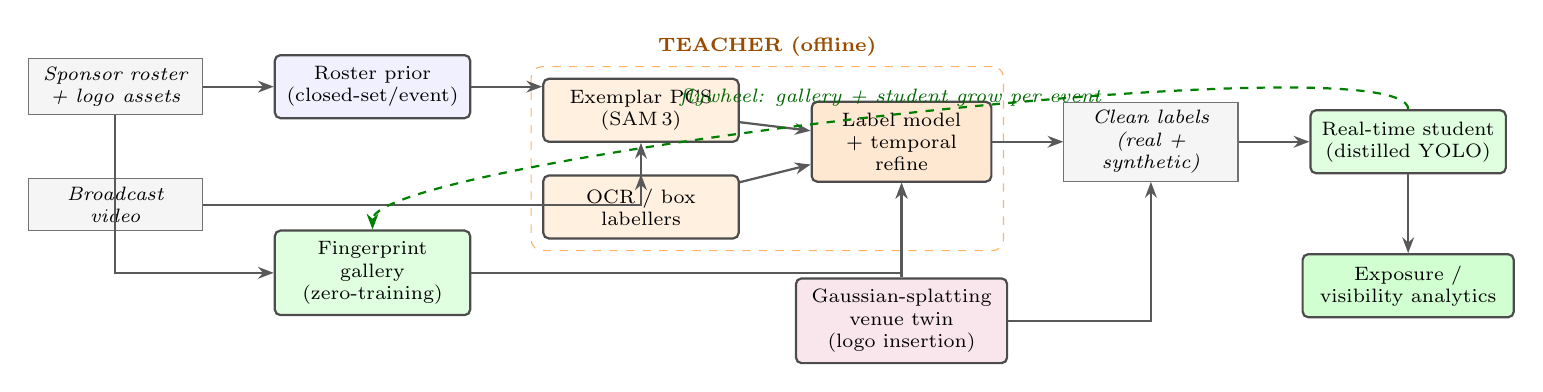
\begin{tikzpicture}[node distance=6mm and 9mm]
  % inputs
  \node[data] (roster) {Sponsor roster\\+ logo assets};
  \node[data, below=8mm of roster] (video) {Broadcast\\video};

  % roster prior + gallery
  \node[blk, right=of roster] (prior) {Roster prior\\(closed-set/event)};
  \node[stud, below=14mm of prior] (gallery) {Fingerprint gallery\\(zero-training)};

  % teacher block
  \node[teach, right=of prior, yshift=-3mm] (pcs) {Exemplar PCS\\(SAM\,3)};
  \node[teach, below=4mm of pcs] (ocr) {OCR / box\\labellers};
  \node[blk, right=of pcs, yshift=-4mm, fill=orange!18, text width=20mm]
       (lm) {Label model\\+ temporal\\refine};

  % twin
  \node[blk, below=12mm of lm, fill=purple!10, text width=24mm]
       (twin) {Gaussian-splatting\\venue twin\\(logo insertion)};

  % clean labels + student
  \node[data, right=of lm] (labels) {Clean labels\\(real + synthetic)};
  \node[stud, right=of labels] (student) {Real-time student\\(distilled YOLO)};
  \node[blk, below=10mm of student, fill=green!18, text width=24mm]
       (analytics) {Exposure /\\visibility analytics};

  % teacher grouping box
  \begin{scope}[on background layer]
    \node[draw=orange!60, dashed, rounded corners, fit=(pcs)(ocr)(lm),
          inner sep=4pt, label={[font=\scriptsize\bfseries,orange!60!black]above:TEACHER (offline)}] {};
  \end{scope}

  % arrows
  \draw[arr] (roster) -- (prior);
  \draw[arr] (roster) |- (gallery);
  \draw[arr] (video) -| (pcs);
  \draw[arr] (video) -| (ocr);
  \draw[arr] (prior) -- (pcs.west|-prior);
  \draw[arr] (pcs) -- (lm);
  \draw[arr] (ocr) -- (lm);
  \draw[arr] (gallery) -| (lm);
  \draw[arr] (twin) -- (lm);
  \draw[arr] (lm) -- (labels);
  \draw[arr] (labels) -- (student);
  \draw[arr] (student) -- (analytics);
  \draw[arr] (twin) -| (labels);

  % flywheel feedback
  \draw[arr, dashed, draw=green!50!black]
       (student.north) .. controls +(0,9mm) and +(0,9mm) .. (gallery.north)
       node[midway, above, font=\scriptsize\itshape, green!40!black] {flywheel: gallery + student grow per event};
\end{tikzpicture}

\caption{\textbf{The cyber-physical data engine.} Per event, the sponsor roster
configures a closed-set prior and a zero-training fingerprint gallery. A heavy
\emph{teacher} (exemplar-prompted PCS + OCR/box labellers, fused by a label model
and temporal refinement) auto-labels the broadcast; a Gaussian-splatting venue
twin injects rare conditions; a light \emph{student} is distilled for real-time
exposure analytics. Each event enlarges the gallery and student (flywheel).}
\label{fig:arch}
\end{figure*}

\subsection{Problem and roster prior (C1)}
Let $\mathcal{B}$ be the universe of brands. Classic detection learns a fixed map
to a closed subset $\mathcal{B}_{\text{train}}\subset\mathcal{B}$. For event $e$
we instead receive its roster $R_e\subset\mathcal{B}$, $|R_e|\!\ll\!|\mathcal{B}|$.
We restrict both labelling and inference to $R_e$: any hypothesis $b\notin R_e$ is
rejected. This is a structural labelling function that removes off-roster false
positives at zero cost (Fig.~\ref{fig:funnel}).

\subsection{Exemplar-to-video auto-labelling (C2)}
For each $b\in R_e$ we hold one or more exemplar images $\{x_b\}$ from existing
assets. We prompt a Promptable Concept Segmentation model
$\mathcal{S}$~\cite{sam3} with $x_b$ on sampled frames; $\mathcal{S}$ segments and
\emph{tracks} every instance ``like $x_b$'' through the clip, yielding masks,
boxes and track ids tagged with $b$. A single exemplar per brand thus labels an
entire broadcast, replacing thousands of manual boxes.

\subsection{Weak-supervision label model (C3)}
Each frame is examined by heterogeneous weak labellers: (i)~PCS exemplar masks;
(ii)~an open-vocabulary box detector; (iii)~scene-text/OCR grounding reading the
brand name; (iv)~gallery embedding match; (v)~temporal track propagation; and
(vi)~the roster prior. A label model aggregates them per candidate region into a
denoised label and confidence (Fig.~\ref{fig:labelmodel}). Agreement above a
threshold is accepted; disagreement is routed to light human review
(active learning).

\subsection{Temporal track refinement}
Following~\cite{trackrefine}, detections are linked into bidirectional tracks.
Long, stable tracks are trusted and \emph{back-propagated} to recover
false-negative frames; short, flickering tracks are discarded. Temporal coherence
acts as label-free supervision and is iterated.

\subsection{Gaussian-splatting venue twin (C4)}
We reconstruct the venue from broadcast footage as a 3D Gaussian-splatting
scene~\cite{gsdata}, then insert \emph{real} logo textures onto boards/jerseys
with lighting-aware compositing~\cite{d3dr} and 6-DoF randomisation
(Fig.~\ref{fig:twin}). Because the background is the real scene and only logos are
synthetic, labels are pixel-perfect while the domain gap stays small. The twin
specifically supplies rare conditions (steep angles, occlusion, glare, rain).

\subsection{Multimodal logo fingerprint (C5)}
Identity is a gallery lookup over a fingerprint
$f(\cdot)=[\,\phi_{\text{vis}}\;\Vert\;\phi_{\text{txt}}\;\Vert\;\phi_{\text{col}}\,]$:
a visual embedding, an OCR text string, and a colour signature. Text disambiguates
visually similar marks; colour adds a cheap prior. A new brand is added by
inserting one fingerprint---\emph{no training}.

\subsection{Distillation and the flywheel (C6)}
Teacher labels (real + twin) distill a real-time student detector (YOLO-class).
Per event the roster reconfigures the gallery, the teacher labels, the student is
updated, and reviewed hard cases re-enter training---so accuracy grows with the
number of processed events.

% ----- secondary method figures (side by side) ------------------------------
\begin{figure}[t]
\centering
% Fig. 2 — Roster prior funnel (C1)
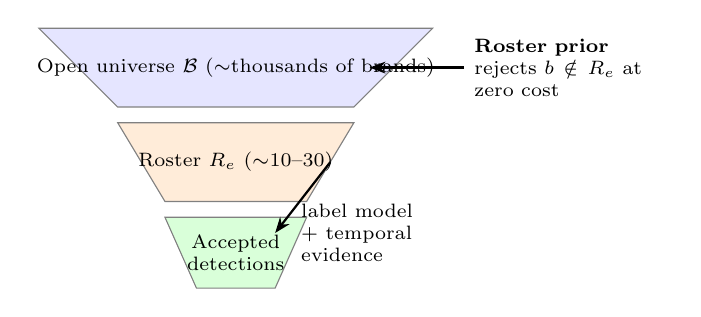
\begin{tikzpicture}[font=\scriptsize]
  % funnel trapezoids
  \fill[blue!10, draw=black!50] (0,0) -- (5,0) -- (4,-1) -- (1,-1) -- cycle;
  \node at (2.5,-0.5) {Open universe $\mathcal{B}$ ($\sim$thousands of brands)};

  \fill[orange!15, draw=black!50] (1,-1.2) -- (4,-1.2) -- (3.4,-2.2) -- (1.6,-2.2) -- cycle;
  \node at (2.5,-1.7) {Roster $R_e$ ($\sim$10--30)};

  \fill[green!15, draw=black!50] (1.6,-2.4) -- (3.4,-2.4) -- (3.0,-3.3) -- (2.0,-3.3) -- cycle;
  \node[align=center] at (2.5,-2.85) {Accepted\\detections};

  % arrows / labels
  \draw[-{Stealth[length=2mm]}, thick] (5.4,-0.5) -- (4.2,-0.5)
       node[right=12mm, align=left, text width=24mm]
       {\textbf{Roster prior}\\rejects $b\notin R_e$ at zero cost};
  \draw[-{Stealth[length=2mm]}, thick] (3.7,-1.7) -- (3.0,-2.6)
       node[right=2mm, align=left, text width=22mm]
       {label model\\+ temporal\\evidence};
\end{tikzpicture}

\caption{\textbf{Roster prior as a funnel (C1).} The known per-event roster turns
open-world recognition into closed-set-per-event, pruning off-roster hypotheses
before they become false positives.}
\label{fig:funnel}
\end{figure}

\begin{figure}[t]
\centering
% Fig. 3 — Weak-supervision label model (C3)
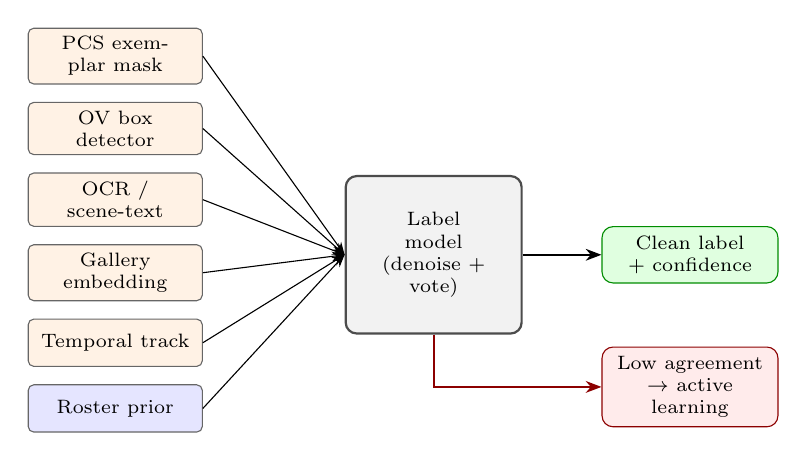
\begin{tikzpicture}[font=\scriptsize, node distance=2.2mm and 10mm,
  lab/.style={rectangle, rounded corners=2pt, draw=black!60, fill=orange!10,
              align=center, inner sep=3pt, text width=20mm, minimum height=6mm}]
  \node[lab] (a) {PCS exemplar mask};
  \node[lab, below=of a] (b) {OV box detector};
  \node[lab, below=of b] (c) {OCR / scene-text};
  \node[lab, below=of c] (d) {Gallery embedding};
  \node[lab, below=of d] (e) {Temporal track};
  \node[lab, below=of e, fill=blue!10] (f) {Roster prior};

  \node[rectangle, rounded corners, draw=black!70, thick, fill=gray!10,
        right=18mm of c, yshift=-7mm, align=center, text width=20mm,
        minimum height=20mm] (lm) {Label\\model\\(denoise +\\vote)};

  \node[rectangle, rounded corners, draw=green!55!black, fill=green!12,
        right=of lm, align=center, text width=20mm] (out) {Clean label\\+ confidence};
  \node[rectangle, rounded corners, draw=red!55!black, fill=red!8,
        below=8mm of out, align=center, text width=20mm] (al) {Low agreement\\$\rightarrow$ active learning};

  \foreach \n in {a,b,c,d,e,f}{\draw[-{Stealth[length=1.6mm]}] (\n.east) -- (lm.west);}
  \draw[-{Stealth[length=2mm]}, thick] (lm) -- (out);
  \draw[-{Stealth[length=2mm]}, thick, red!55!black] (lm.south) |- (al.west);
\end{tikzpicture}

\caption{\textbf{Weak-supervision label model (C3).} Heterogeneous foundation-model
labellers vote per candidate region; the label model denoises consensus into a
clean label and confidence, with low-agreement regions sent to active learning.}
\label{fig:labelmodel}
\end{figure}

\begin{figure}[t]
\centering
% Fig. 4 — Gaussian-splatting venue twin pipeline (C4)
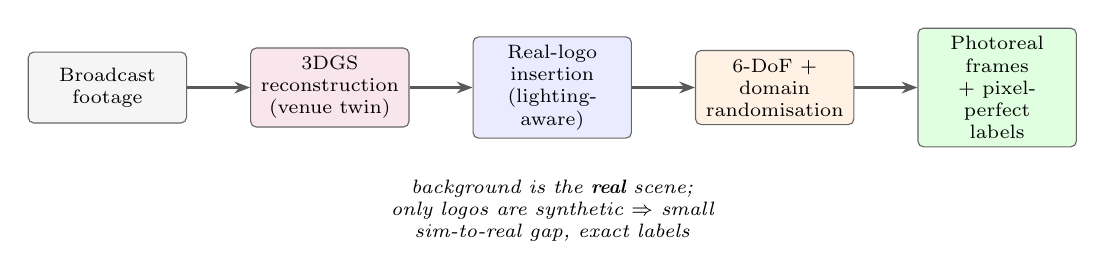
\begin{tikzpicture}[font=\scriptsize, node distance=8mm,
  st/.style={rectangle, rounded corners=2pt, draw=black!60, align=center,
             inner sep=3pt, text width=18mm, minimum height=9mm}]
  \node[st, fill=gray!8]    (foot) {Broadcast\\footage};
  \node[st, fill=purple!10, right=of foot] (gs) {3DGS\\reconstruction\\(venue twin)};
  \node[st, fill=blue!8, right=of gs]   (ins) {Real-logo\\insertion\\(lighting-aware)};
  \node[st, fill=orange!10, right=of ins] (dr) {6-DoF +\\domain\\randomisation};
  \node[st, fill=green!12, right=of dr]  (out) {Photoreal frames\\+ pixel-perfect\\labels};

  \draw[arr] (foot) -- (gs);
  \draw[arr] (gs) -- (ins);
  \draw[arr] (ins) -- (dr);
  \draw[arr] (dr) -- (out);

  \node[align=center, below=4mm of ins, font=\scriptsize\itshape, text width=44mm]
    {background is the \textbf{real} scene; only logos are synthetic
     $\Rightarrow$ small sim-to-real gap, exact labels};
\end{tikzpicture}

\caption{\textbf{Gaussian-splatting venue twin (C4).} Real footage is reconstructed
as a 3DGS scene; real logos are inserted with lighting-aware compositing and 6-DoF
randomisation, yielding photoreal frames with pixel-perfect labels.}
\label{fig:twin}
\end{figure}

% ============================================================================
\section{Experiments}
\label{sec:exp}

\subsection{Setup}
\textbf{Data.} Rugby-league broadcasts across \TODOnum{$N$} matches and varied
lighting. A held-out, hand-annotated \emph{gold} test set is used \emph{only} for
evaluation (never for training). An \emph{open-set} split withholds
\TODOnum{$k$} brands to test zero-training addition. Synthetic data comes from
copy-paste, diffusion compositing, and the venue twin.

\textbf{Implementation.} PCS backbone~\cite{sam3}; OCR/text labeller via
LocateAnything~\cite{locateanything} (research-only); student is a distilled
YOLO. Frame sampling, roster, thresholds and the fingerprint are as in our public
data-engine code. Seeds and versions are pinned for reproducibility.

\subsection{Baselines}
(1)~Supervised closed-set YOLO trained on $N_{\text{lab}}$ hand-labelled frames
(cost upper bound); (2)~Grounded-SAM auto-labels (foundation-model only, no roster
/ label model); (3)~open-set retrieval / template matching; (4)~\textbf{Ours}
(full) and its ablations.

\subsection{Metrics}
Detection mAP@.5 and mAP@.5:.95; per-brand precision/recall; open-set accuracy on
withheld brands and false-positive rate on non-sponsors; \emph{annotation
efficiency} (mAP vs.\ number of manual labels); analytics error on exposure-time
and visibility-\% against ground truth; and student FPS.

\subsection{Main results}
\begin{table}[t]
\centering
\caption{Detection and analytics (gold test set). Numbers are placeholders.}
\label{tab:main}
\renewcommand{\arraystretch}{1.15}
\setlength{\tabcolsep}{3pt}
\begin{tabular}{lccccc}
\toprule
Method & Manual & mAP@.5 & mAP & Open-set & Exp.\ err \\
       & labels &        & @.5:.95 & acc.\   & (s) \\
\midrule
Supervised YOLO     & \TODOnum{$10^3$} & \TODOnum{--} & \TODOnum{--} & n/a          & \TODOnum{--} \\
Grounded-SAM auto   & \TODOnum{0}      & \TODOnum{--} & \TODOnum{--} & \TODOnum{--} & \TODOnum{--} \\
Open-set retrieval  & \TODOnum{0}      & \TODOnum{--} & \TODOnum{--} & \TODOnum{--} & \TODOnum{--} \\
\textbf{Ours (full)}& \TODOnum{$\sim$0}& \TODOnum{--} & \TODOnum{--} & \TODOnum{--} & \TODOnum{--} \\
\bottomrule
\end{tabular}
\end{table}

\subsection{Annotation efficiency}
Fig.~\ref{fig:eff} plots mAP against the number of manual labels: our engine
reaches the supervised plateau with a small fraction of the labels---the central
practical claim.

\begin{figure}[t]
\centering
% Fig. 5 — Annotation efficiency curve (ILLUSTRATIVE placeholder data)
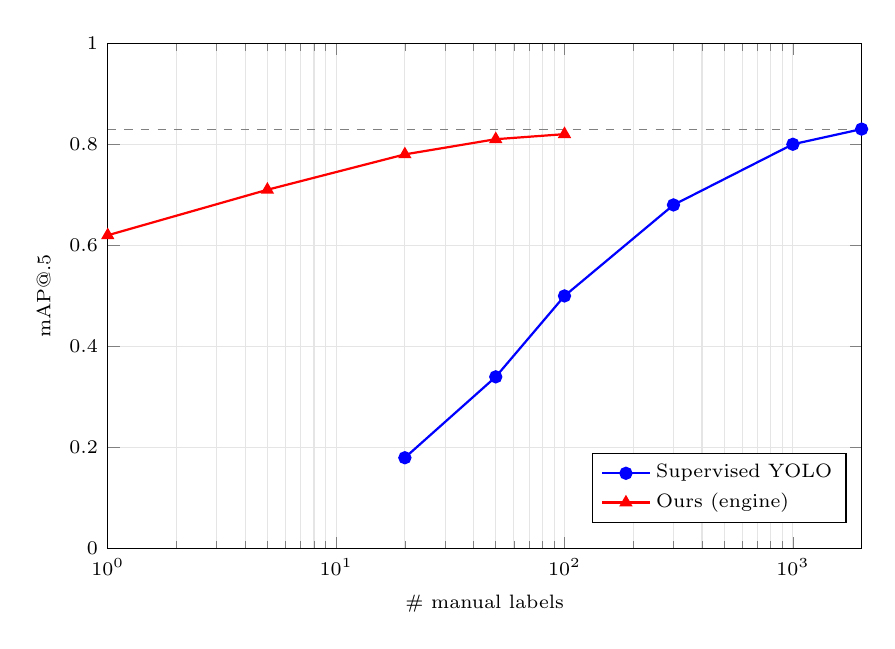
\begin{tikzpicture}
\begin{axis}[
  width=0.92\columnwidth, height=0.66\columnwidth,
  xlabel={\# manual labels}, ylabel={mAP@.5},
  xmode=log, log basis x=10,
  xmin=1, xmax=2000, ymin=0, ymax=1,
  grid=both, grid style={gray!20}, tick label style={font=\scriptsize},
  label style={font=\scriptsize},
  legend style={font=\scriptsize, at={(0.98,0.05)}, anchor=south east},
  legend cell align=left,
]
% supervised baseline (needs many labels) -- PLACEHOLDER
\addplot[mark=*, thick, blue] coordinates
  {(20,0.18)(50,0.34)(100,0.50)(300,0.68)(1000,0.80)(2000,0.83)};
\addlegendentry{Supervised YOLO}
% ours (auto-label, few/no manual) -- PLACEHOLDER
\addplot[mark=triangle*, thick, red] coordinates
  {(1,0.62)(5,0.71)(20,0.78)(50,0.81)(100,0.82)};
\addlegendentry{Ours (engine)}
% supervised plateau guide
\addplot[dashed, black!50, forget plot] coordinates {(1,0.83)(2000,0.83)};
\end{axis}
\end{tikzpicture}

\caption{\textbf{Annotation efficiency (illustrative).} mAP vs.\ number of manual
labels. The engine approaches the supervised plateau at a fraction of the cost;
final curves use measured values.}
\label{fig:eff}
\end{figure}

\subsection{Ablations}
Fig.~\ref{fig:ablation} isolates each contribution: removing the roster prior
(C1), the label model / temporal refinement (C3), the venue twin (C4), and the
text/colour fingerprint channels (C5). The flywheel (C6) is shown as accuracy vs.\
number of processed events.

\begin{figure}[t]
\centering
% Fig. 6 — Ablation bar chart (ILLUSTRATIVE placeholder data)
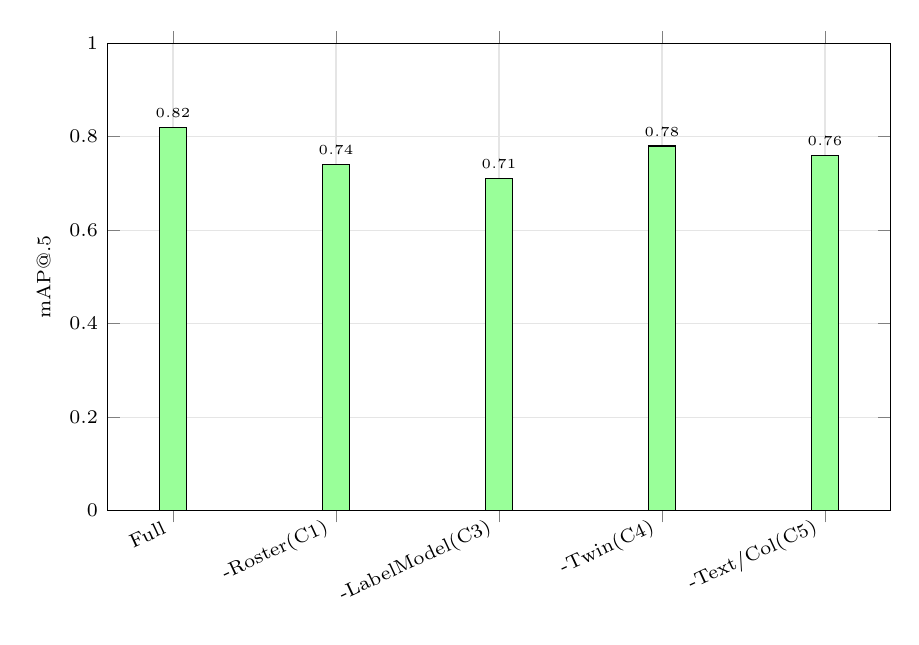
\begin{tikzpicture}
\begin{axis}[
  width=0.95\columnwidth, height=0.62\columnwidth,
  ybar, bar width=10pt,
  ymin=0, ymax=1, ylabel={mAP@.5},
  symbolic x coords={Full,-Roster(C1),-LabelModel(C3),-Twin(C4),-Text/Col(C5)},
  xtick=data, x tick label style={rotate=25, anchor=east, font=\scriptsize},
  tick label style={font=\scriptsize}, label style={font=\scriptsize},
  nodes near coords, nodes near coords style={font=\tiny},
  grid=both, grid style={gray!20},
]
% PLACEHOLDER deltas -- replace with measured values
\addplot[fill=green!40] coordinates
  {(Full,0.82) (-Roster(C1),0.74) (-LabelModel(C3),0.71)
   (-Twin(C4),0.78) (-Text/Col(C5),0.76)};
\end{axis}
\end{tikzpicture}

\caption{\textbf{Ablation (illustrative).} Contribution of each component to
mAP@.5. Replace bar heights with measured deltas.}
\label{fig:ablation}
\end{figure}

% ============================================================================
\section{Discussion, Limitations, Ethics}
The engine assumes the roster is known---true for professional competitions but
not for arbitrary footage. SAM\,3 and 3DGS are recent; tracking of tiny/blurred
logos and twin fidelity need per-domain validation, and synthetic sources must be
mixed with real auto-labels to avoid sim-to-real drift. LocateAnything is
research-only; a commercial deployment must swap it for a permissively licensed
detector. Ethically, the system analyses brand exposure, not people; player and
spectator privacy is preserved by not performing person identification.

% ============================================================================
\section{Conclusion}
Re-framing sponsor-logo detection around three free signals---existing assets, the
known roster, and temporal redundancy---turns an annotation-bound task into a
self-improving cyber-physical data engine. Coupling exemplar-to-video
foundation-model labelling, weak-supervision fusion, a Gaussian-splatting venue
twin, and a multimodal fingerprint yields an annotation-free, sport-agnostic,
expandable analytics system. Future work: live per-event adaptation and
render-and-verify self-supervision.

% ============================================================================
\bibliographystyle{IEEEtran}
\bibliography{refs}

\end{document}
